\chapter{Resultados.}\label{sec:resultados}

\paragraph{}En este capítulo se van a mostrar de forma resumida los resultados del proyecto,
así como el resultado del prototipo. Resultados que por diseño, están pensados para
poder ser utilizados como plantillas o como punto de partida para futuros proyectos.

\section{Aplicación Rpi Weather}\label{sec:rpiweather}

\paragraph{}La aplicación Rpi Weather es una aplicación sencilla que cumple su función
decorativa e informativa. Una vez fijada una ciudad, nos muestra una breve información
del estado climatológico de esa ciudad. Además, nos muestra la fecha y hora local.

\paragraph{}Está pensada para su uso en pequeños dispositivos IoT de salón, a modo de
sencilla estación meteorológica decorativa.

\begin{figure}[H]
	\centering
	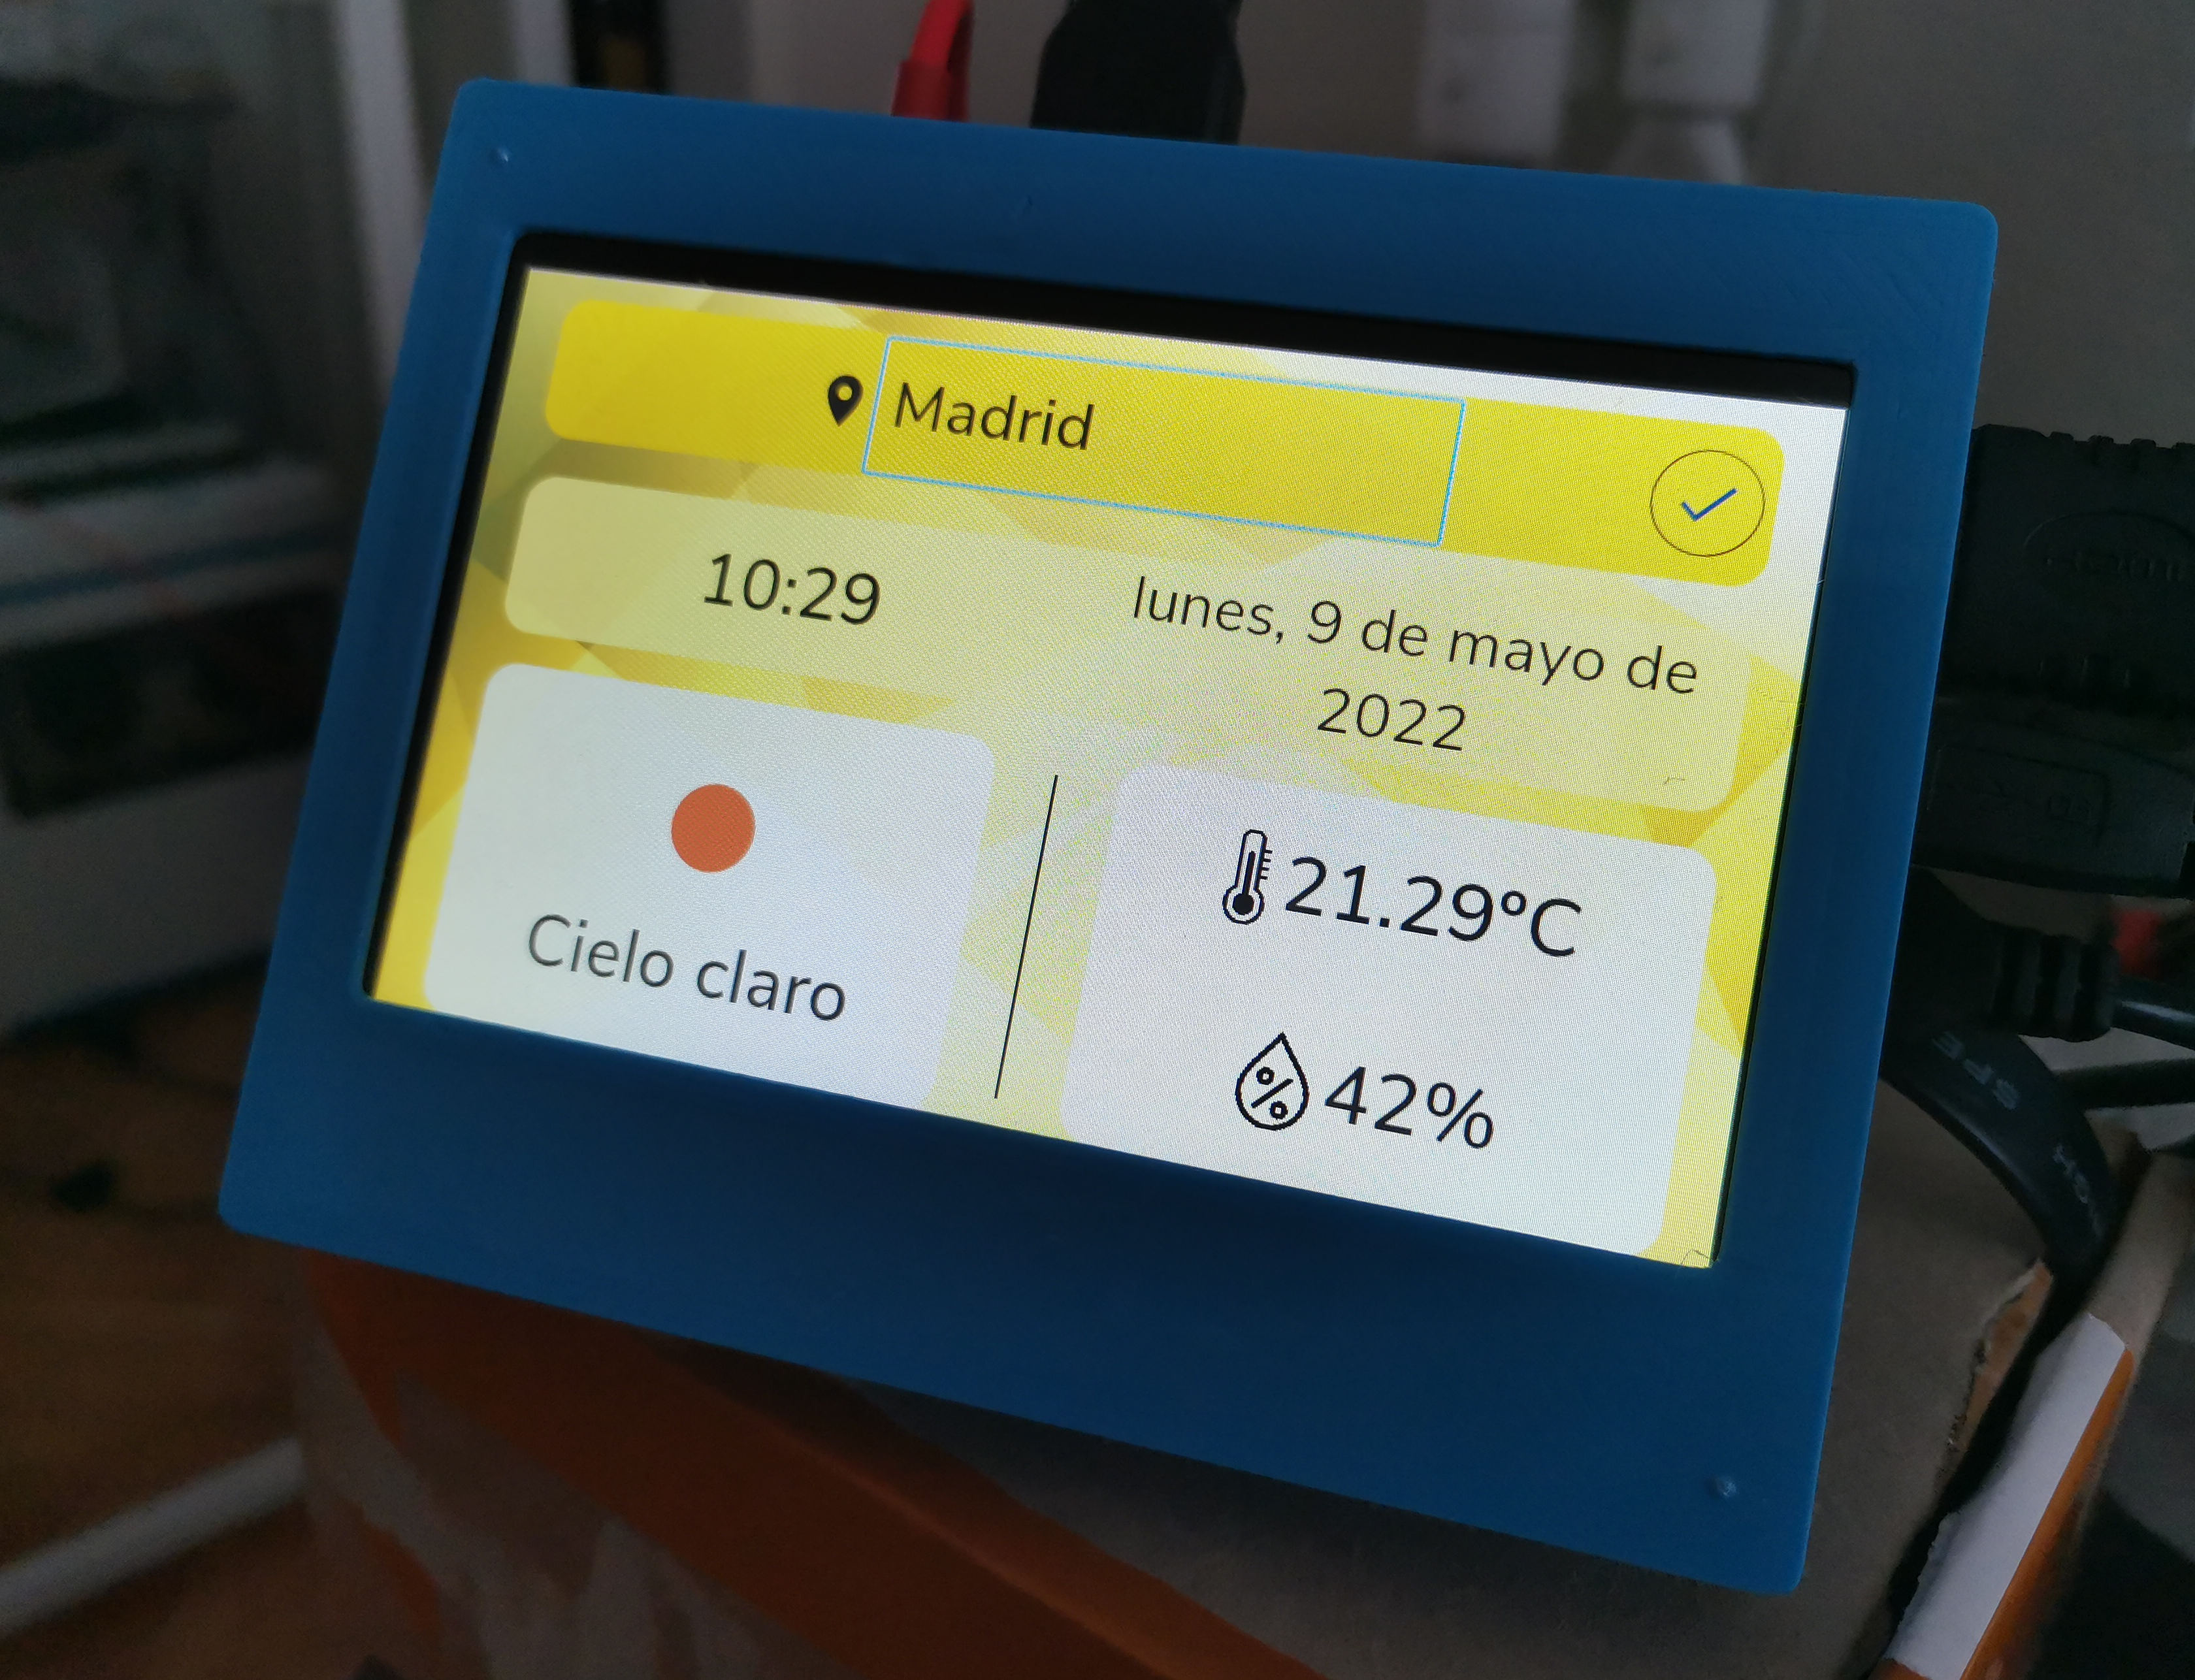
\includegraphics[width=0.70\linewidth]{imgs/app1}
	\caption[Rpi Weather]{Rpi Weather.}
	\label{img:rpi-weather-app}
\end{figure}

\section{Sistema Operativo FlutterPi}\label{sec:flutterpi}

\paragraph{}El sistema operativo Flutter Pi es un sistema basado en el kernel de Linux,
generado con Yocto con las siguientes características principales:

\begin{itemize}
    \item Compatible con Raspberry Pi (ARMv7) de 32 bits.
    \item Incluye el motor embebido de Flutter.
    \item Incluye drivers gráficos de Vulkan con simulación de switfshaders.
    \item Incluye la configuración de una red Wi-Fi.
    \item Compatibilidad con pantalla LCD 5" táctil a través de HDMI.
    \item Servicio de arranque automático de la aplicación Flutter configurada.
    \item Servicio de levantamiento de interfaz Wi-Fi y conexión automática con
    punto de acceso configurado.
\end{itemize}

\section{El Prototipo}\label{sec:prototipo}

\paragraph{}El aspecto exterior del prototipo, está caracterizado por su carcasa impresa
en 3D. La carcasa está divida modularmente en tres partes diferentes: la carcasa de la
pantalla LCD 5", la carcasa de la Raspberry Pi 3B+ y el soporte inclinado. Quiero
agradecer al usuario \href{https://www.thingiverse.com/thing:3444545}{ywabiko} de
Thingiverse su tiempo y dedicación en diseñar el modelo.

\begin{figure}[H]
	\centering
	\subfigure[Trasera del prototipo]{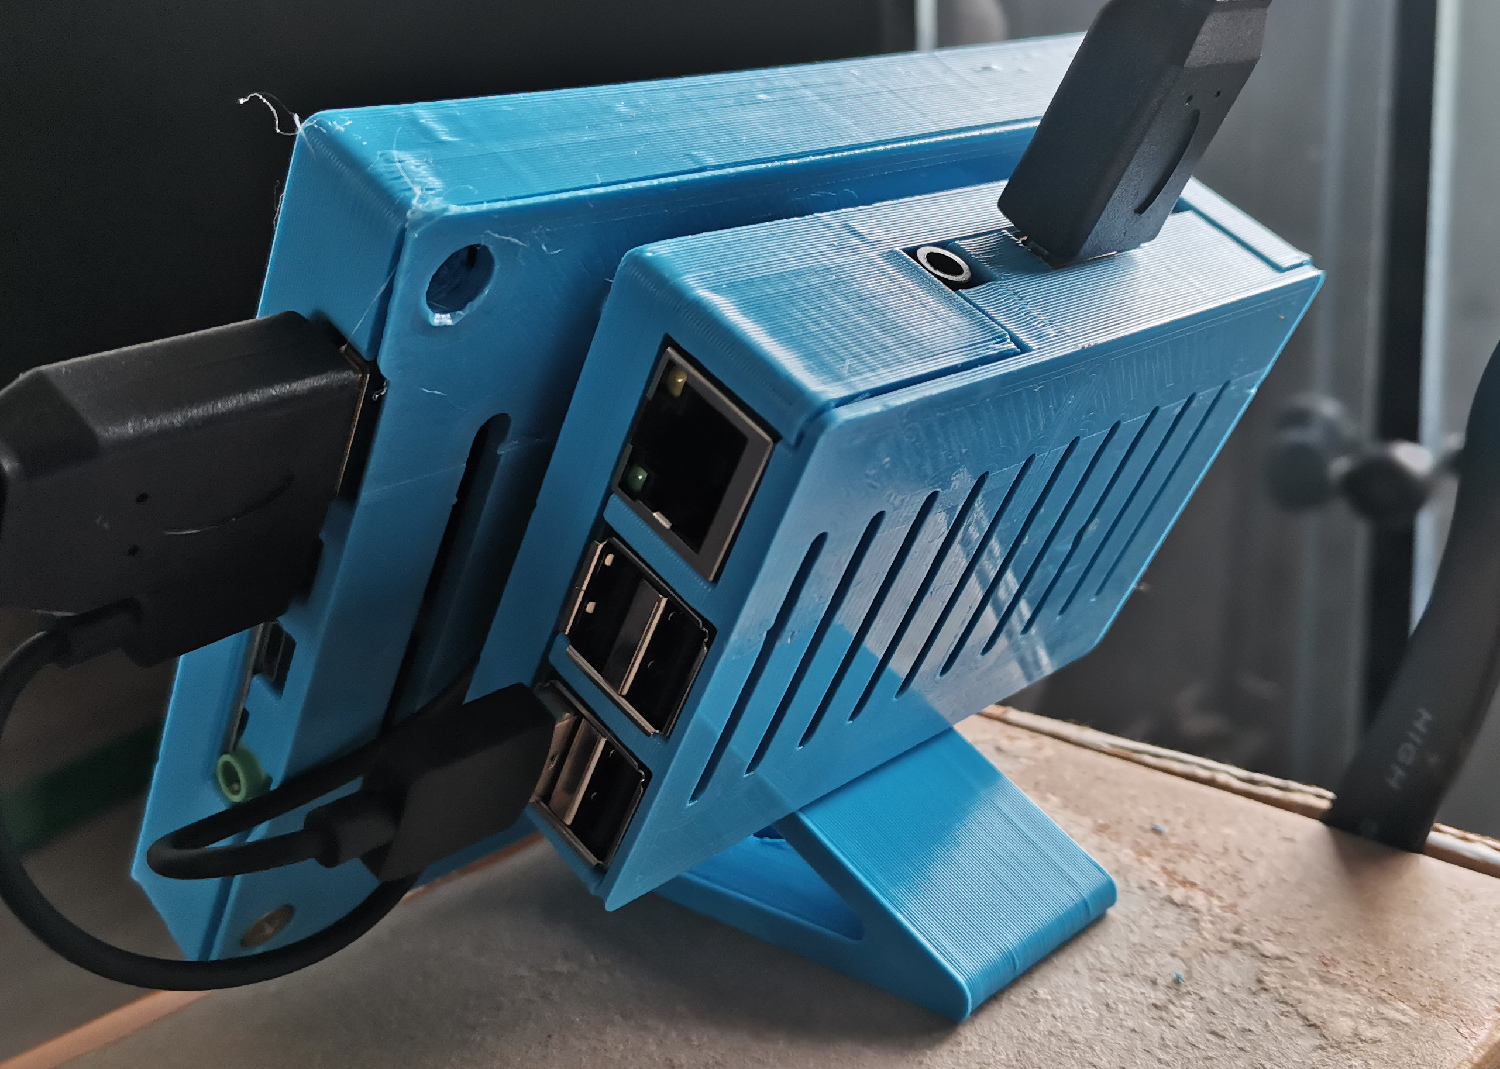
\includegraphics[width=0.4\linewidth]{imgs/proto-back1}}
    \subfigure[Trasera del prototipo]{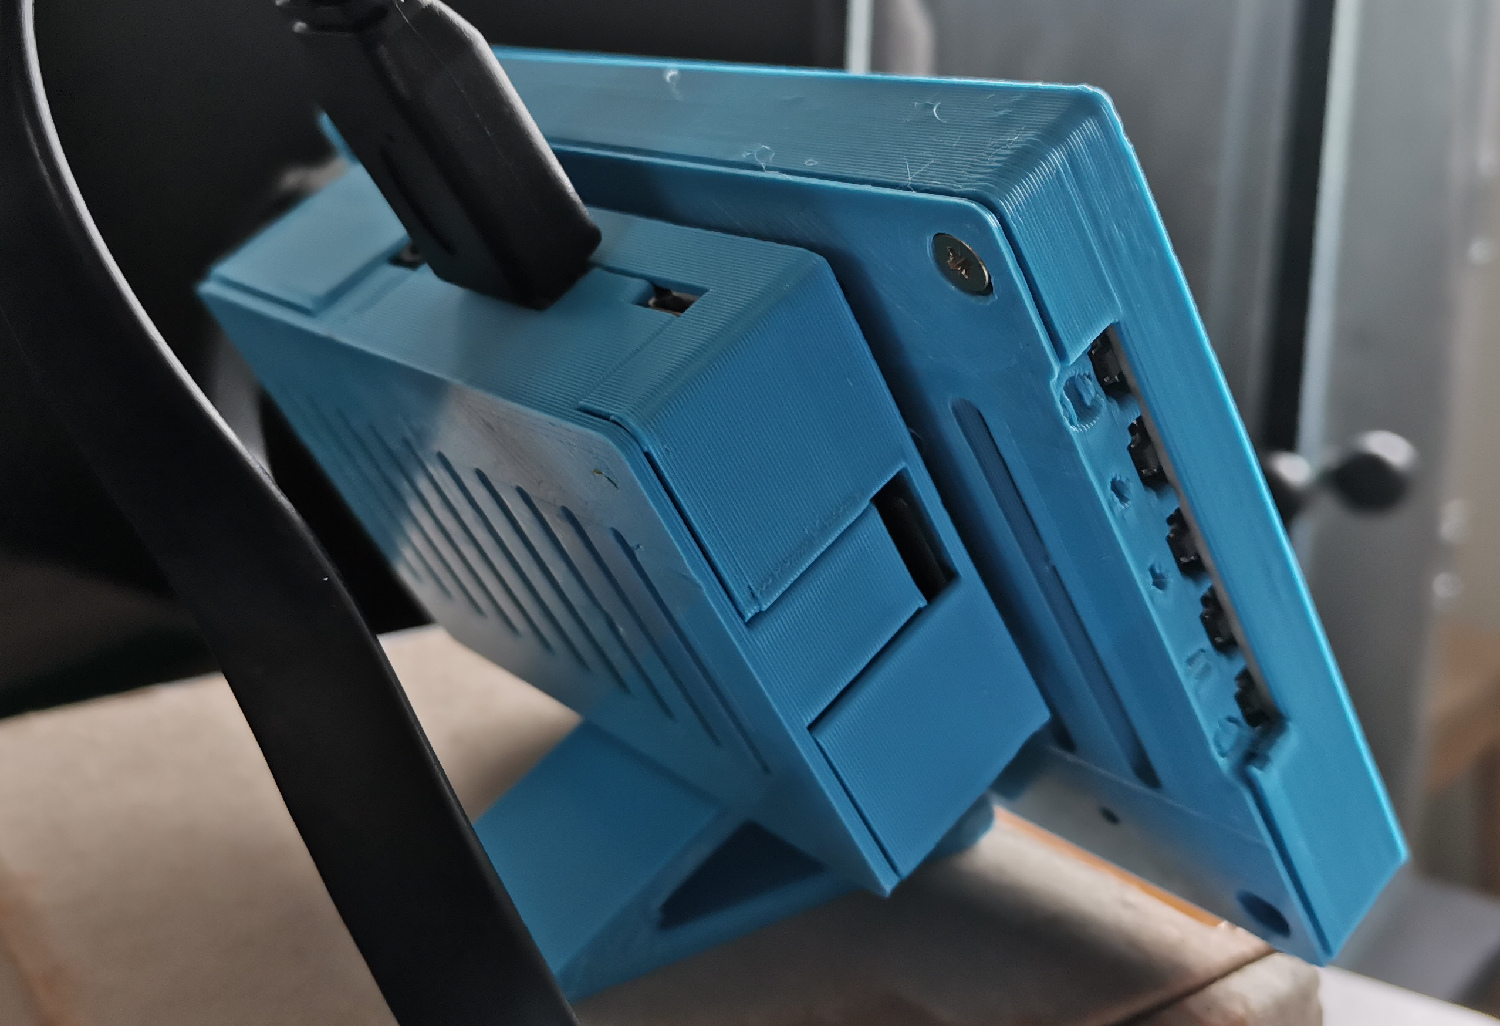
\includegraphics[width=0.4\linewidth]{imgs/proto-back2}}
    \subfigure[Frontal del prototipo]{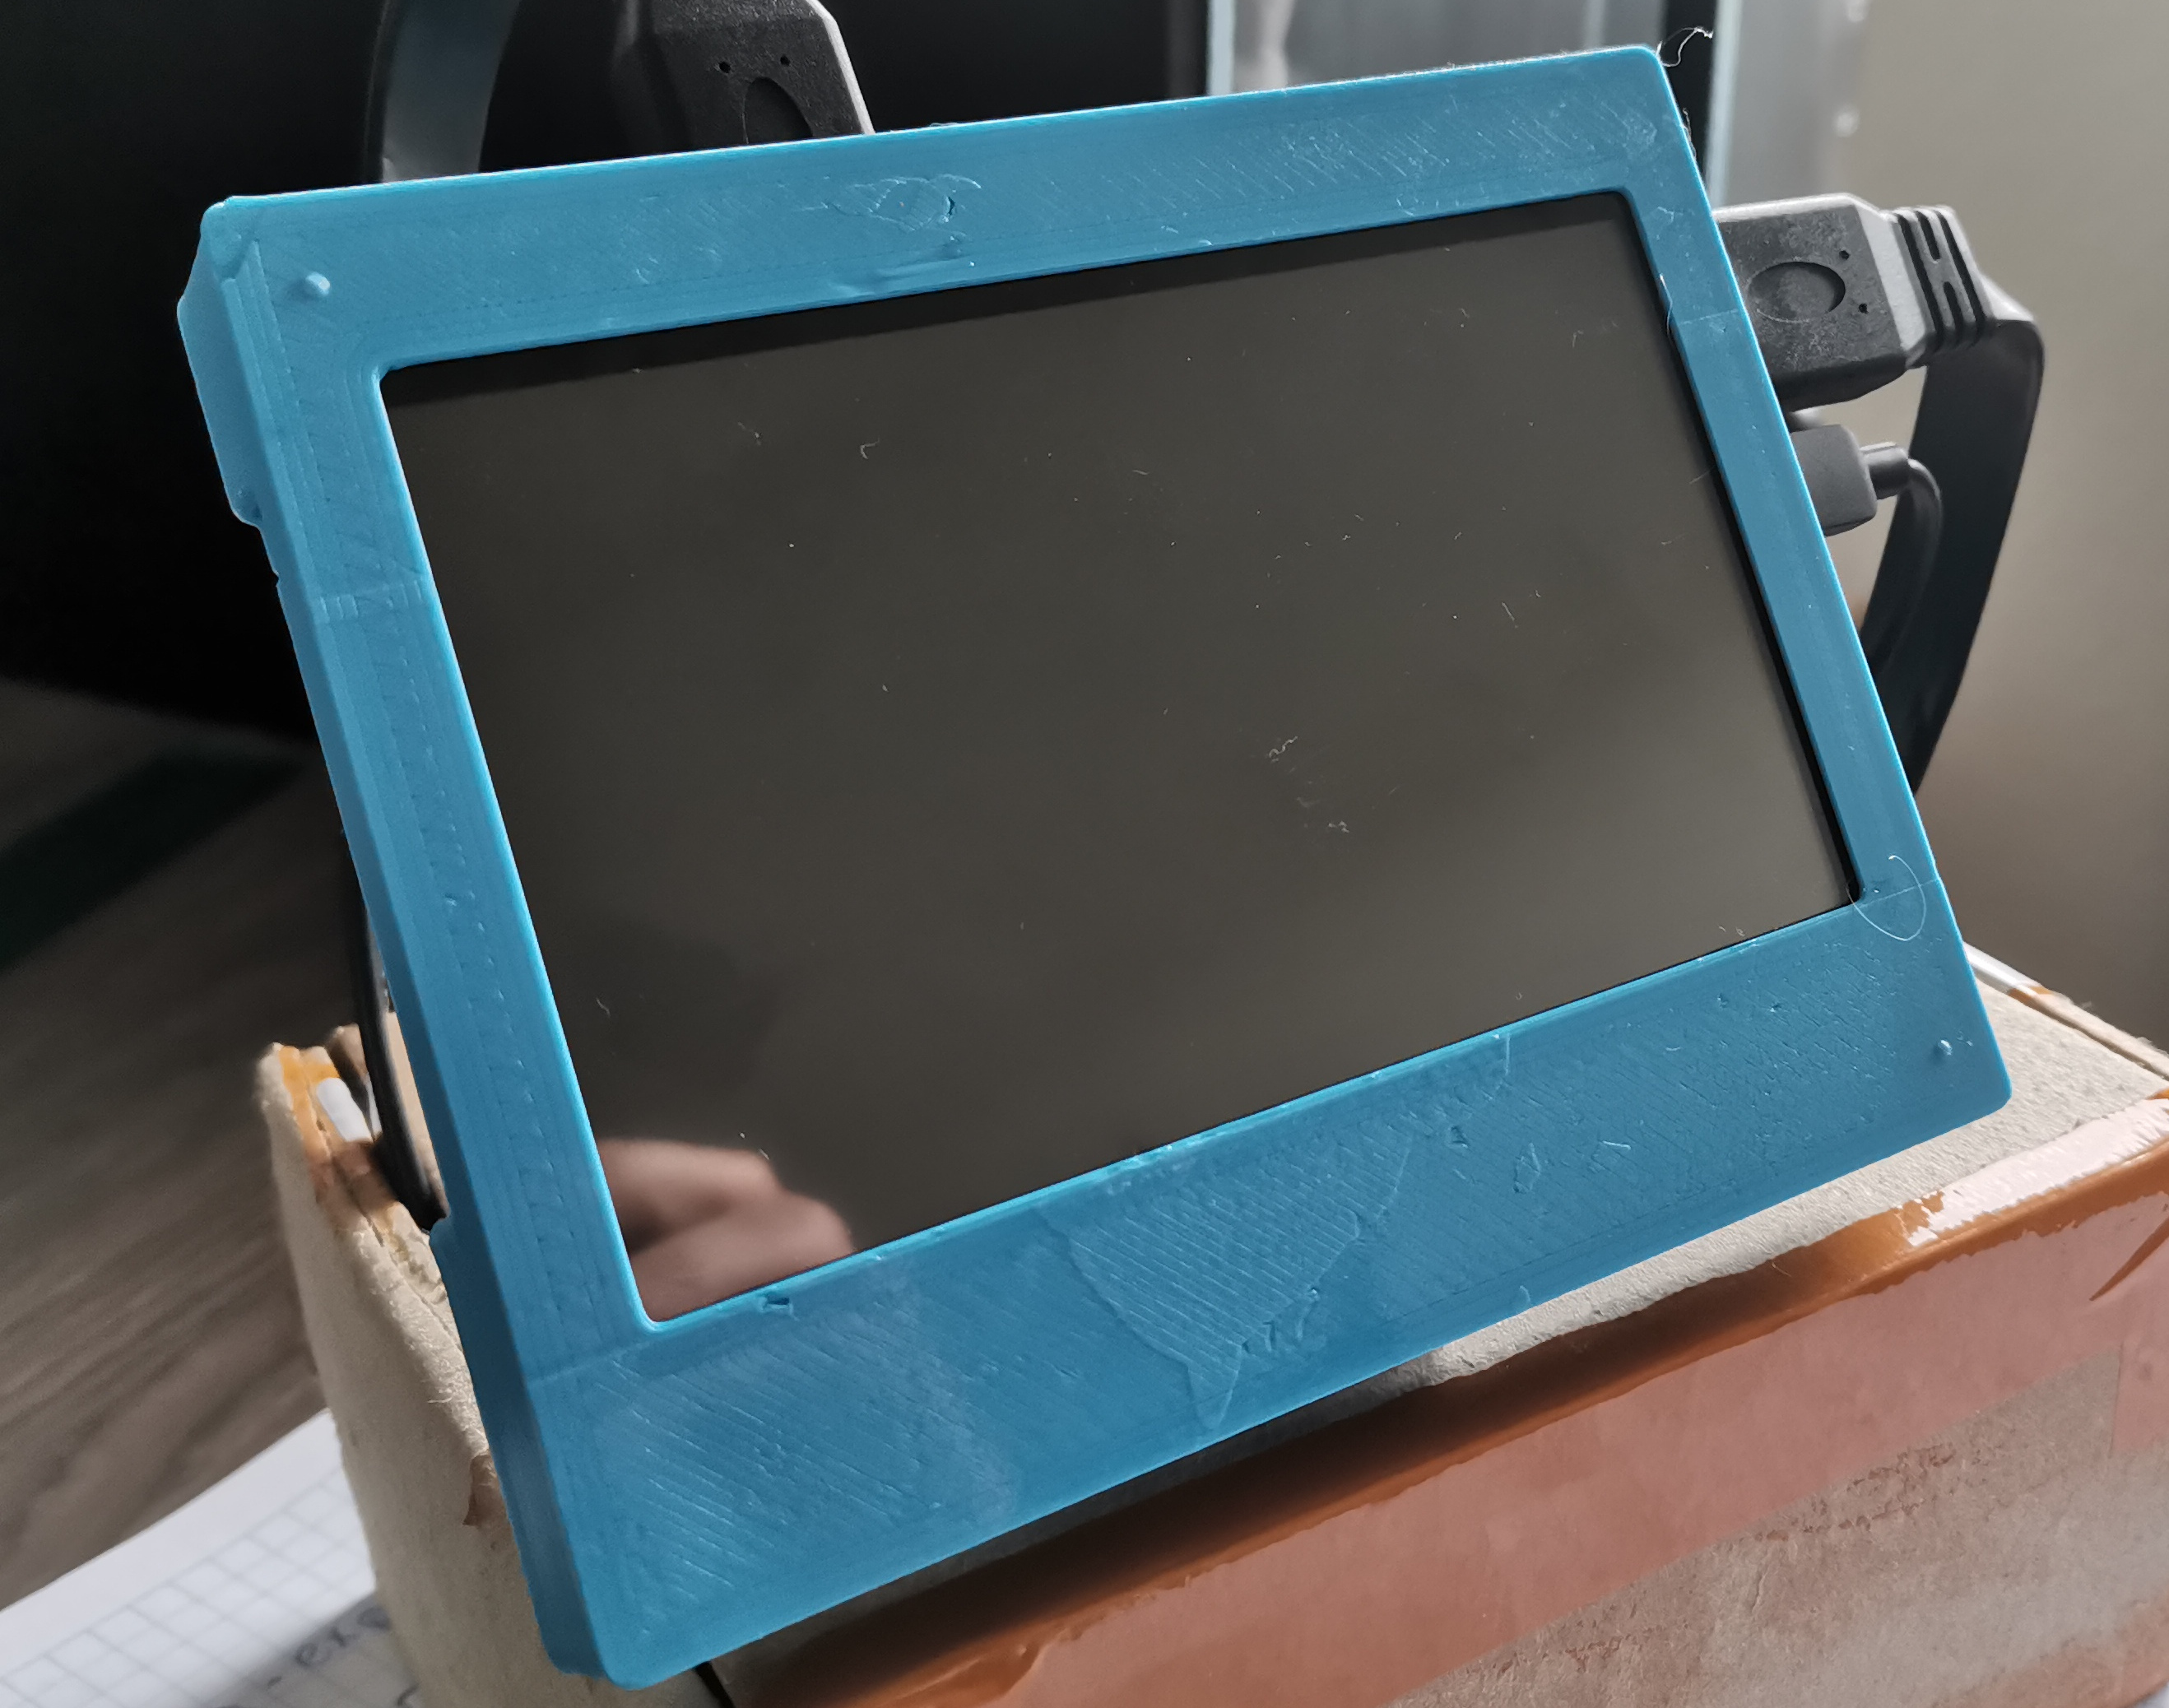
\includegraphics[width=0.4\linewidth]{imgs/proto-front}}
	\caption[Prototipo]{Diferentes vistas del prototipo.}
	\label{img:proto-views}
\end{figure}

%las referencias a artículos se ponen con \cite,
%las referencias a glosario \gls,
%y las referencias a ecuaciones \eqref
%las referencias a imgenes, tablas o figuras o secciones
% se ponen con \ref (sólo número) o con \hyperref[sec:X]{text}
